\documentclass{beamer}

\mode<presentation>
{
  \usetheme{default}      % or try Darmstadt, Madrid, Warsaw, ...
  \usecolortheme{default} % or try albatross, beaver, crane, ...
  \usefonttheme{serif}  % or try serif, structurebold, ...
  \setbeamertemplate{navigation symbols}{}
  \setbeamertemplate{caption}[numbered]
}

\newcommand{\Prob}{\text{Prob}}
\newcommand{\bx}{\mathbf{x}}
\newcommand{\bphi}{\pmb{\phi}}
\newcommand{\btheta}{\pmb{\theta}}
\newcommand{\given}{\, | \,}
\DeclareMathOperator*{\argmax}{arg\,max}

\begin{document}


%%%%FRAME
\begin{frame}{Common Terminology}
    \begin{exampleblock}{Vocabulary}
        The set $V = \{w_1,w_2,\ldots, w_V\}$ of all the \textit{words} or \textit{tokens}.
    \end{exampleblock}
        \begin{itemize}
            \item \textbf{Common Crawl (uncased)} 42B tokens, 1.9M vocab.
            \item \textbf{Common Crawl (cased)} 840B tokens, 2.2M vocab.
            \item \textbf{Twitter} 2B tweets, 27B tokens, 1.2M vocab
            \item \textbf{Wikipedia 2014 + Gigaword 5} 6B tokens 400K vocab
            \item \textbf{arXiv.org} 1,000,295 vocab.arxmliv.txt
        \end{itemize}

        \begin{exampleblock}{Labels or Classes}
            The set of labels $\{y^{(1)},y^{(2)},\ldots, y^{(n)}\}$\\
            In the example these were: \textbf{Definitions, Examples, Propositions, etc}.
        \end{exampleblock}


\end{frame}

\begin{frame}{Bag of Words Model}
    Represent a document, email, tweet as a vector $\bx=(x_1,\ldots, x_V)$
    \begin{columns}[T]
        \begin{column}{0.6\textwidth}
            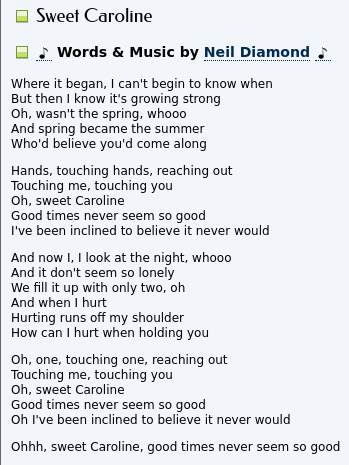
\includegraphics[width=0.9\textwidth]{sweet_caroline_lyrics.png}
        \end{column}
        \begin{column}{0.4\textwidth}
            \begin{tabular}{|c|l|c|}
                \hline
                \hline
                $V$ & UNK& Freq. \\
                \hline
                \hline
                23 & oh&6\\
                \hline
                4500 & touching&6\\
                \hline
                10 & good&6\\
                \hline
                80 & never&5\\
                \hline
                50 & seem&4\\
                \hline
                38 & believe&3\\
                \hline
                99 & sweet&3\\
                \hline
                43 & caroline&3\\
                \hline
                30 & time&3\\
                \hline
                90 &know&2\\
                \hline
                54& spring&2\\
                \hline
                897& whooo&2\\
                \hline
                230 & hand&2\\
                \hline
                654 & reaching&2\\
                \hline
            \end{tabular}
        \end{column}
    \end{columns}
\end{frame}

\begin{frame}{Na\"ive Bayes}
    Suppose we have a long list of $N$ labeled documents $$\{(\bx^{(i)},y^{(i)}) :\ i = 1,\ldots, N \}$$
        And $\bx^{(i)}\given y^{(i)} $ has a Multinomial distribution with parameters $\bphi = (\phi_1,\ldots, \phi_V)$ 
        $$\Prob(\bx\given y;\bphi) = \frac{(\sum_{j=1}^V x_j)!}{x_1!\cdots x_V!}\  \prod_{j=1}^V \phi_j^{x_j}$$

        We are interested in:
        $$\Prob(y\given \bx) = \frac{\Prob(y)\  \Prob(\bx \given y; \bphi)}{\Prob(\bx)}\propto \Prob(\bx, y,\bphi)$$
        Since:
        $$\Prob(\bx,y; \bphi) = \Prob(y) \ \Prob(\bx \given y; \bphi)$$

\end{frame}


%%%%FRAME
\begin{frame}{Na\"ive Bayes (Prediction)}
     We choose the label that maximizes the joint probability:
     $$\hat y = \argmax_y\left\{ \Prob(\bx, y: \bphi)\right \}$$
     Equivalently:
     $$\hat y = \argmax_y\left\{ \log \Prob(\bx\given y: \bphi) + \log\Prob(y)\right\}$$
     {\color{green}Reminder:} $\displaystyle \Prob(\bx\given y;\bphi) = B(\bx) \prod_{j=1}^V \phi_j^{x_j}$\\
     Subtituting inside the log:
     $$= \log B(\bx) + \btheta\cdot f(\bx, y)$$
     
\end{frame}


%%%%FRAME
\begin{frame}{Na\"ive Bayes (Estimation)}
    We use the labels to find $\bphi$ as follows:
     $$\Prob(y^{(i)}\given \bx^{(j)} ) = \delta_{i,j}$$
\end{frame}

\begin{frame}
Nobody in this seminar has that (and I'm happy) but the hard part is the Data Mining.
Machine learning is fun, it's high level, rewarding and very little coding unless you want to do things from scratch.\\

    Human language can be ambiguous
    \begin{itemize}
            \item The Pope's baby steps on gays.
            \item Scientist study whales from space.
    \end{itemize}
\end{frame}

\begin{frame}{Similarity based representations}
    ``You shall know a word by the company it keeps''\\[5mm]
    \hspace*\fill{\small John R. Firth}

\end{frame}

\begin{frame}
    \title{Distributional Similarity based representations}
    If $w_t$ is the word we care about then:
    $$Jexp(\theta) = \prod_{t=1}^T \prod_{\substack{|j|\leq m\\ j\neq 0}} \Prob(w_{t+j}| w_t; \theta)$$
    $$J(\theta) = \frac 1T \sum_{t=1}^T \sum_{\substack{|j|\leq m\\ j\neq 0}}\log \Prob(w_{t+j}| w_t; \theta)$$
\end{frame}

%%%%FRAME
\begin{frame}{How we  choose the word}
     $$p(o|c) = \frac{\exp(u_0^T v_c)}{\sum_{w=1}^V \exp(u_w^Tv_c}$$
\end{frame}


%%%%FRAME
\begin{frame}{GloVe Project}
    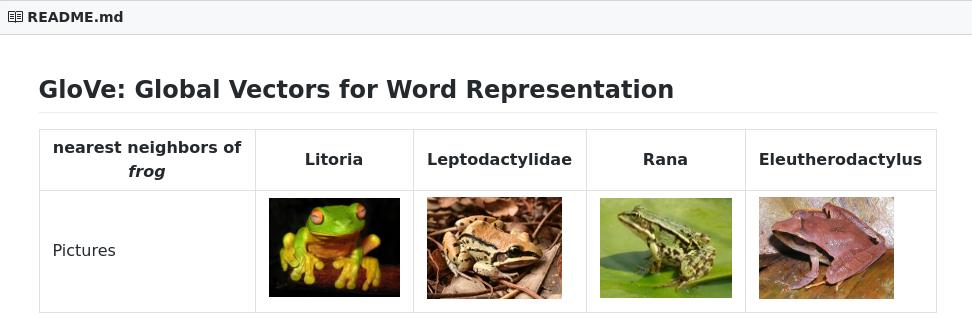
\includegraphics[width=\textwidth]{Glove_github_small.png}

\begin{figure}
   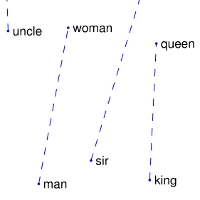
\includegraphics[width=0.29\textwidth]{man_woman_small.jpg}
   \hfill
   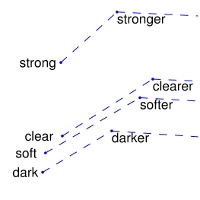
\includegraphics[width=0.29\textwidth]{comparative_superlative_small.jpg}
   \hfill
   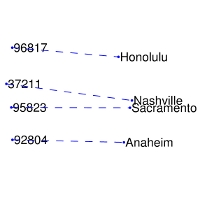
\includegraphics[width=0.29\textwidth]{city_zip_small.jpg}
\end{figure}

\end{frame}


\end{document}
